\renewcommand*{\arraystretch}{1.1}

\noindent\begin{tabularx}{17cm}{|>{\small \sf}c|X|}
	\hline
	query    & Interactive / complex / 12 \\ \hline
%
	title       & Expert search \\ \hline
%
    pattern     & \hfill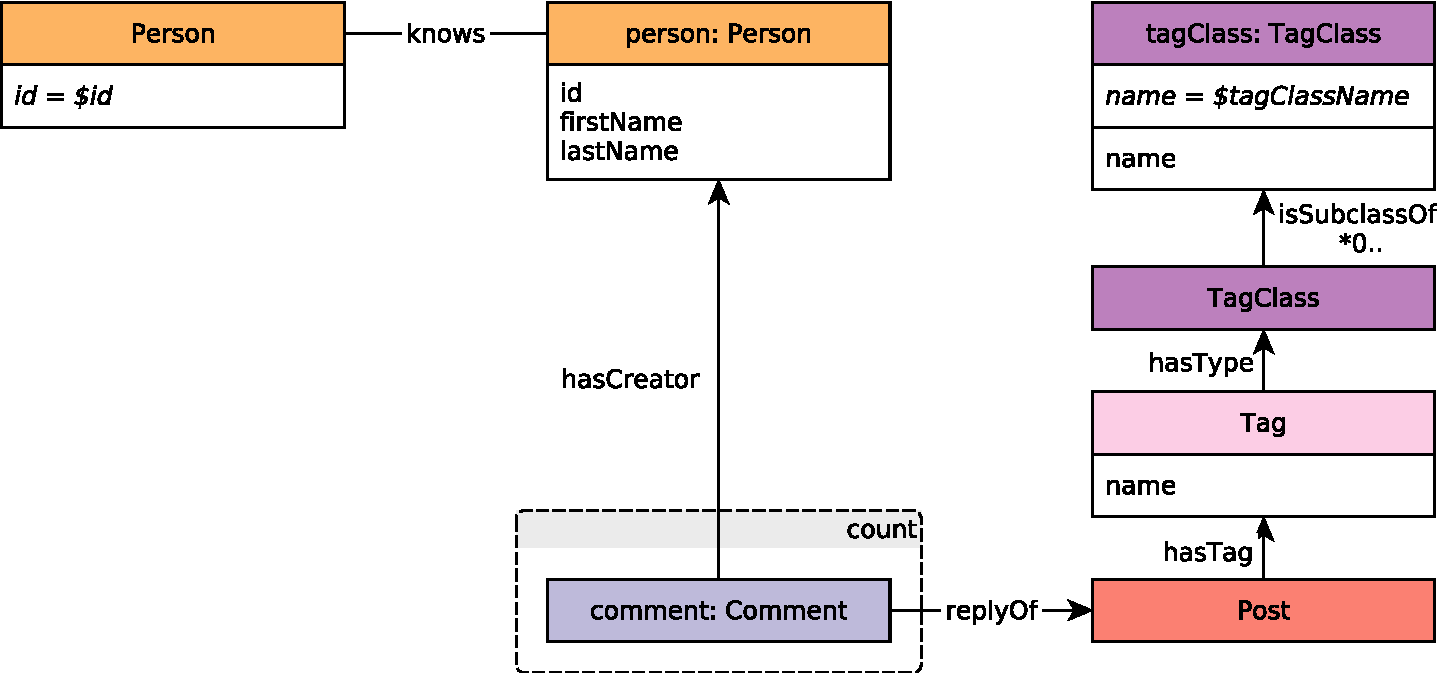
\includegraphics[scale=\patternscale,margin=0cm .2cm]{patterns/interactive-complex-read-12}\hfill\vadjust{} \\ \hline
%
	desc. & Given a start Person, find the Comments that this Person's friends made
in reply to Posts, considering only those Comments that are immediate
(1-hop) replies to Posts, not the transitive (multi-hop) case. Only
consider Posts with a Tag in a given TagClass or in a descendent of that
TagClass. Count the number of these reply Comments, and collect the Tags
that were attached to the Posts they replied to, but only collect Tags
with the given TagClass or with a descendant of that TagClass Return
Persons with at least one reply, the reply count, and the collection of
Tags.
 \\ \hline
%
	
%
	params  &
	\vspace{1.1ex}{\begin{tabularx}{14.66cm}{|c|M|m{2cm}|Y|} \hline
	\cellcolor{parameter} \color{white} \footnotesize $\mathsf{1}$ & \varname{Person.id} & \cellcolor{gray!20} \vartype{ID} &  \\ \hline
	\cellcolor{parameter} \color{white} \footnotesize $\mathsf{2}$ & \varname{TagClass.name} & \cellcolor{gray!20} \vartype{String} &  \\ \hline
	\end{tabularx}}\vspace{1.1ex} \\ \hline
%
	
	result      &
	\vspace{1.1ex}{\begin{tabularx}{14.66cm}{|c|M|m{2cm}|c|Y|} \hline
	\cellcolor{result} \color{white} \footnotesize $\mathsf{1}$ & \varname{Person.id} & \cellcolor{gray!20} \vartype{ID} &
	    \texttt{R} &
	     \\ \hline
	\cellcolor{result} \color{white} \footnotesize $\mathsf{2}$ & \varname{Person.firstName} & \cellcolor{gray!20} \vartype{String} &
	    \texttt{R} &
	     \\ \hline
	\cellcolor{result} \color{white} \footnotesize $\mathsf{3}$ & \varname{Person.lastName} & \cellcolor{gray!20} \vartype{String} &
	    \texttt{R} &
	     \\ \hline
	\cellcolor{result} \color{white} \footnotesize $\mathsf{4}$ & \varname{\{Tag.name\}} & \cellcolor{gray!20} \vartype{\{String\}} &
	    \texttt{R} &
	     \\ \hline
	\cellcolor{result} \color{white} \footnotesize $\mathsf{5}$ & \varname{count} & \cellcolor{gray!20} \vartype{32-bit Integer} &
	    \texttt{A} &
	    number of reply Comments \\ \hline
	\end{tabularx}}\vspace{1.1ex} \\ \hline
	
%
	sort        &
	\vspace{1.1ex}{\begin{tabular}{|c|l|c|} \hline
	\cellcolor{sort} \color{white} \footnotesize $\mathsf{1}$ & \varname{count} & \cellcolor{gray!20} $\desc$ \\ \hline
	\cellcolor{sort} \color{white} \footnotesize $\mathsf{2}$ & \varname{Person.id} & \cellcolor{gray!20} $\asc$ \\ \hline
	\end{tabular}}\vspace{1.1ex} \\ \hline
	%
	limit       & 20 \\ \hline
	%
	CPs &
	\multicolumn{1}{>{\raggedright}l|}{
	  \chokepoint{1.5}, 
	  \chokepoint{3.3}, 
	  \chokepoint{7.2}, 
	  \chokepoint{7.3}
	  } \\ \hline
	%
    relevance &
      \small This query looks for paths of length three, starting at a Person, moving to its friends, the to their Comments and
ending at the Post the Comments are replying. The chain from original post to the reply is transitive. The traversal
may be initiated at either end, the system may note that this is a tree, hence leaf to root is always best. Additionally,
a hash table can be built from either end, e.g. from the friends of self, from the tags in the category, from the or
other.
 \\ \hline%
\end{tabularx}
\vspace{2ex}